\documentclass[11pt]{article}
\usepackage[letterpaper]{geometry} %So margins are not their default huge
\usepackage{geometry}
\usepackage{dsfont}
\usepackage{amsmath}
\usepackage{framed}
\usepackage{booktabs}
\usepackage{tabularx}
\usepackage{graphicx}
\usepackage{caption}
\usepackage{subcaption}
\usepackage{pdfpages}
\usepackage{pdflscape}
\usepackage{threeparttable}
\usepackage{makecell}
\usepackage{longtable}
\usepackage{multirow,multicol}
\usepackage{setspace}\spacing{1.5}
\geometry{left=1in, right=1in, top=1in, bottom=1in}
%\usepackage{tgbonum}
\renewcommand{\familydefault}{\rmdefault}
\rmfamily
\usepackage[parfill]{parskip}    % Activate to begin paragraphs with an empty line
\usepackage{graphicx}
%\usepackage[round, sort&compress, authoryear]{natbib}
\usepackage{float, amsmath, mathtools, amsfonts, amssymb, bm, amsthm, commath, mathrsfs, xcolor, verbatim, tikz, enumerate, tabu, hhline, longtable, pdfpages, hyperref, mdframed}
\usepackage[all]{hypcap}
\setlength\textheight{648pt}
\DeclareMathOperator*{\argmax}{argmax}
\begin{document}
\title{RAISE: Effects of Limiting Low-Skilled Immigrants on Wages and Government Revenues}
\author{Ruby Zhang}
\maketitle

\begin{abstract}
  In light of President's Trump new RAISE Act, which awards visas based on merit and will cut down low-skilled immigrants, this paper aims to look at whether wages increase if such an immigration shock were to take place. By modelling a simple capital-less economy with low and high-skilled workers, results show that low-skilled workers are better off in terms of wages and welfare, while high-skilled workers (whose immigration has not been affected) are worse off over time \footnote{All code to run the model is public and open-source at https://github.com/rzhang15/immigration.git}. However, they are still better off than low-skilled workers. Despite decreasing inequality, the new anti-immigration shock also decreases output growth and government revenue growth from taxation. By determining labor endogenously, this model allows agents to optimize freely unlike previous literature. Therefore, this model implies that while there is reasoning behind the Act to improve the welfare of low-skilled native workers, it will come at a cost to overall economic development.
\end{abstract}

\pagebreak

\section{Introduction}

In early August of this year, President Trump announced his support for a new immigration policy that would cut the number of legal immigrants in half \cite{nytimes}. The new bill, known as the Reforming American Immigration for Strong Employment (RAISE) Act, would screen visa applicants using a merit system that favors young, highly-educated applicants with high-paying job offers \cite{timemag}. The White House released an official statement that stated their main claims for supporting the RAISE act \cite{whitehouse}:
\begin{enumerate}
  \item Most immigrants that enter the United States are low and unskilled workers, who are more likely to receive welfare benefits.
  \item The influx of low-skilled immigrants depress wages for low-skilled Americans.
  \item The influx of low-skilled immigrants puts pressure on tax-payers and the government budget.
\end{enumerate}

On the hand, proponents of immigration claim that net immigration would boost economic output and create new jobs since immigrants are themselves consumers. In addition to output, supporters claim that wages, prices, innovation, and even government revenue all benefit from immigration \cite{fortune}.

Despite the different arguments cited by both sides, studies by George Borjas have found partial truths in both claims \cite{politico}. Borjas found that skill groups with the largest number of immigrants will suffer a wage decrease (in this case, low-skilled workers). However, the economic pie grows due to increase in production and labor, which in turn make employers better off. Furthermore, the increase in taxpayers also offsets government spending. Borjas concludes that immigration has caused more of a redistribution in wealth rather than a direct effect, and that increasing high-skilled immigration can lead everyone to be better off.

Similar to Borjas, most economists have studied the empirical and theoretical impacts of an influx of immigrants on the economy. Many economists also test the net effects of immigration regardless of skill level, such as when looking at net innovation in the economy.

In light of the RAISE Act and the motivations behind its creation, this paper aims to answer the main question: does severely limiting low-skilled immigrants raise wages for low-skilled native workers and generate more government revenue? Rather than studying the effects of increased immigration, this paper assumes a steady immigration rate and a subsequent shock once the RAISE Act is implemented. The differentiation between high-skilled and low-skilled workers in this paper's model will allow the effects of the RAISE Act on consumption and wages for each worker to be isolated. However, this capital-less economy with only one type of consumption good greatly simplifies the actual production sector and labor interactions between different skilled workers.

\section{Literature Review}

There have been numerous empirical studies on the economic impacts of immigration, with many not finding evidence of one-to-one crowding out effects of immigration. Longhi, Nijkamp, and Poot (2005) \cite{longhi} found that for every 10$\%$ increase of immigrants in the work force, earnings for natives change anywhere between $-2\%$ and $2\%$. Hercowitz and Yashiv (2002) \cite{hercowitz} found that immigrants, consuming as soon as they arrive, increase the demand for goods and services more than their production. Thus, more jobs and opportunities are created with the arrival of immigrants.

On the other hand, once labor skills are disagregated, many studies find a negative impact of U.S. immigration on low-skilled workers. Ottaviano and Peri (2012) \cite{ottaviano} found that on average in the past two decades, earnings rose by $0.6\%$ for native workers due to a balanced influx of low-skill and high-skill workers. However, the negative impact has been to earlier immigrants, whose wage was decreased by $6.7\%$, with higher figures for earlier immigrants with less education. Cortes (2008) \cite{cortes} looked at immigrant stocks by city and concluded that a 10$\%$ incrase in immigrant share in the low-skill workforce cuts wages by 1 to 1.5$\%$. He found no significant effect on high-skill services.

A big discrepancy between papers has been whether or not capital scales and adjusts to offer new jobs. Borjas (2003) \cite{borjas03} assumes that capital stock does not adjust to more labor, leading to the conclusion that there is a decrease in wages for laborers of all education level (i.e. skill type), with a next decrease in $3.2\%$ in wages when calibrated to U.S. immigration. On the other hand, Ottaviano and Peri (2012) \cite{ottaviano} assume labor-adjusting capital stock, and they found that native workers of all skills had a nonnegative wage change while foreign workers of all skill levels had a decrease in wages. Borjas (2014) \cite{borjas14} readjusts his model to consider both adjusting and non-adjusting capital stock, finding that there is still a decrease in wages for low-skilled workers even with capital adjustment. Both authors use a skill cell method that groups immigrants into certain skill levels and calibrates elasticities that determine wages between the skill cells.

Some papers also looked at data generated from natural experiments when large numbers of immigrants entered a territory in a certain time frame. Clemens (2013) \cite{clemens} used employment data from North Carolina offices and found that certain immigrant and native labor markets were separate, thus there was not a crowding out effect in terms of employment. Friedberg (2001) \cite{Friedberg} used the flow of Soviet Jewish immigrants in the early 1990's and found that the 12$\%$ labor expansion increased wages by $8.9\%$ for those already working.

Other studies looking specifically at innovation and productivity have that immigrants increase productivity and new creations. Using census data, Peri (2012) \cite{Peri} found that immigration increased both output per unit of labor and capital input. Kerr and Lincoln (2010) \cite{kerr} and Moser et al. (2013) \cite{moser} found an increase in patents by H-1B holders and after the immigration of chemists post-WWII, respectively.

Lisenkova (2013) \cite{lisenkova} looked at the impacts of immigration on public finances with an overlapping generations and competitive general equilibrium framework. The household optimized a stream of consumption, and she utilized different skill levels with similar elasticities of subsitution to determine labor and wage levels. She found that a mass reduction in immigration reduces the GDP by $11\%$, and that labor income tax needs to be increased by $2\%$ in order to keep a balanced government budget constraint.

\section{Model Specification}
Since the goal of this paper is to look at the effects of different skilled immigration when acting through wages, the model is a capital-less economy that has two types of workers: high-skilled and low-skilled. All agents only live for one period, and there are no intertemporal transfers or investment assets. Therefore, the only difference between periods is the number of high-skilled and low-skilled workers, which is affected by the native growth rate and immigration. Unlike previous models, agents will be maximizing over both consumption and labor (thus it is endogenously determined).

  \subsection{Household}

  Every period, each agent chooses both consumption and labor in order to maximize their utility (note that labor causes disutility). We do not impose the constraint of labor being a maximum of one unit. We will utilize a separable utility function that models the utility of consumption using constant relative risk aversion (CRRA) and the disutility of labor using a constant Frisch elasticity (CFE). Therefore, the utility function is given as:
  \begin{align*}
    U(c_{i,t}, n_{i,t}) &= \frac{c_{i,t}^{1-\sigma}-1}{1-\sigma}-\frac{n_{i,t}^{1+\frac{1}{\theta}}}{1+\frac{1}{\theta}} \quad \sigma \geq 1, \quad \theta>0, \quad c_{i,t}\geq 0,\quad i\in\{h, l\} \\
    c_{i,t} &= \text{ consumption of a single agent of type $i$ in period t} \\
    n_{i,t} &= \text{ labor of a single agent of type $i$ in period t} \\
    \sigma &= \text{ coefficient of relative risk aversion on consumption}\\
    \theta &= \text{ Frisch elasticity of labor supply}
  \end{align*}

  Since each agent lives for one period, the household budget constraint is $ c_{i,t} = w_{i,t} n_{i,t}$. Agents then maximize according to the following Lagrangian:
  $$ \mathscr{L} = U(c_{i,t}, n_{i,t}) + \lambda(w_{i,t} n_{i,t}-c_{i,t})$$
  Taking the first order conditions, we have the household optimization characterized by the Euler equation:
  $$\lambda = U_c(c_{i,t}, n_{i,t})$$
  $$\lambda w_{i,t}= -U_n(c_{i,t}, n_{i,t})$$
  $$\therefore -\frac{U_n(c_{i,t}, n_{i,t})}{U_c(c_{i,t}, n_{i,t})} = w_{i,t} \Rightarrow  n_{i,t}^{\frac{1}{\theta}} c_{i,t}^\sigma= w_{i,t}$$

  \subsection{Firm}
  There is one representative firm that utilizes two types of labor, high-skilled and low-skilled, with a constant elasticity of substitution in order to produce one type of consumption good. We assume that the share of high-skilled labor is greater than the share of low-skilled labor involved in production. Thus, a constant elasticity of substitution (CES) production function is used for each period:
  \begin{align*}
      Y_t &= A(\alpha N_{h,t}^r + (1-\alpha) N_{l,t}^r )^{\frac{1}{r}} \quad \alpha \in (0.5,1), \quad A>0, \quad r \in (0,1)\\
      A &= \text{ factor of production} \\
      r &= \frac{s-1}{s} \\
      s &= \text{ elasticity of substitution} \\
      \alpha &= \text{ share} \\
      N_{h,t} &= \text{ total high-skilled labor at time } t  \\
      N_{l,t} &= \text{ total low-skilled labor at time } t
  \end{align*}

  Note that we are restricting the elasticity of substitution $s\in(1,\infty)$. Thus, we are assuming that high-skilled and low-skilled labor are substitute rather than complementary goods, though to varying degrees.

  The representative maximized profits every period by choosing the total amount of high-skilled and low-skilled labor to employ with wages $w_{h,t}$ and $w_{l,t}$, respectively:

  $$\max_{N_{h,t},N_{l,t}} Y_t - w_{h,t} N_{h,t} - w_{l,t} N_{l,t}$$

  Taking the first order conditions, we have the firm optimization:
  $$w_{h,t} = A(\alpha N_{h,t}^r + (1-\alpha) N_{l,t}^r )^{\frac{1}{r}-1} \alpha N_{h,t}^{r-1} $$
  $$w_{l,t} = A(\alpha N_{h,t}^r + (1-\alpha) N_{l,t}^r )^{\frac{1}{r}-1} (1-\alpha) N_{l,t}^{r-1} $$

  Note that for both agents, the amount of both low-skilled and high-skilled labor affects the wage if $r\neq 1$ (i.e. not perfect substitutes). Therefore, the change in low-skilled immigration will impact wages for high-skilled and low-skilled workers when the labor is not perfect substitutes (which is assumed to be the case).

  \subsection{Immigration}
  Assume that the initial population of high-skilled and low-skilled workers is given by $p_{h,0}$ and $p_{l,0}$. Let the native growth rate of the population be denoted by $\delta$, and the rates of immigration for high-skilled and low-skilled workers be $\delta_h$ and $\delta_t$, respectively. Then flow of population for every period is:
  $$p_{i,t+1} = p_{i,t}(1+\delta+\delta_i), \quad i\in\{h,l\}$$
  We will model immigration effects of RAISE by adjusting $\delta_i$.

  \subsection{Competitive Equilibrium}
  At each period, the competitive equilibrium is characterized by the allocations $\{c_{i,t}, n_{i,t}\}_{i\in\{h, l\}}$ such that:
  \begin{enumerate}
    \item Each agent maximizes according to the household problem. In other words, $ n_{i,t}^{\frac{1}{\theta}} c_{i,t}^\sigma= w_{i,t}$ where the budget constraint is binding $c_{i,t}=w_{i,t} n_{i,t}$
    \item The firm maximizes profits. In other words:
    $$w_{h,t} = A(\alpha N_{h,t}^r + (1-\alpha) N_{l,t}^r )^{\frac{1}{r}-1} \alpha N_{h,t}^{r-1} $$
    $$w_{l,t} = A(\alpha N_{h,t}^r + (1-\alpha) N_{l,t}^r )^{\frac{1}{r}-1} (1-\alpha) N_{l,t}^{r-1} $$
    \item The labor market clears: $N_{i,t} = p_{i,t} n_{i,t}$
    \item The goods market clears: $Y_t = p_{h,t} c_{h,t}+ p_{l,t} c_{l,t}$
  \end{enumerate}
  Note that we have 9 equations and 8 unknowns, thus one of the conditions is redundant. In fact, the clearing of the goods market is redundant by Walras' law. Please refer to appendix I for the brief proof.

  We can substitute the labor market clearing into the firm optimization, then the household optimization along with the budget constraint. In the end, we have the following system of two equations and two variables to pin down equilibrium labor levels for each type of agent (refer to appendix I for derivation):
  $$ n_{h,t}^{\frac{1+\theta}{\theta}+r(\sigma-1)} = [A(\alpha (p_{h,t} n_{h,t})^r + (1-\alpha) (p_{l,t} n_{l,t})^r )^{\frac{1}{r}-1}]^{1-\sigma} (\alpha p_{h,t}^{r-1})^{1-\sigma}$$
  $$ n_{l,t}^{\frac{1+\theta}{\theta}+r(\sigma-1)} = [A(\alpha (p_{h,t} n_{h,t})^r + (1-\alpha) (p_{l,t} n_{l,t})^r )^{\frac{1}{r}-1}]^{1-\sigma} ((1-\alpha) p_{l,t}^{r-1})^{1-\sigma}$$
  Taking the ratio of the labor of the two types of agents, we have that:
  $$\left(\frac{n_{h,t}}{n_{l,t}}\right)^{\frac{1+\theta}{\theta}+r(\sigma-1)}=\left(\frac{\alpha}{(1-\alpha)}\left(\frac{p_{l,t}}{p_{h,t}}\right)^{1-r}\right)^{1-\sigma}$$

  Note that if $r=1$, i.e. high-skilled and low-skilled labor are perfect substitutes, then the labor ratio is completely independent of the population ratio between the two types of workers and is only dependent on the production share. However, this is not the case since high-skilled labor is generally more specialized and will not be perfectly substitutable with low-skilled labor.

\section{Anti-Immigration Shock Without Taxation}
We will first assume the absence of a government and observe the effects of anti-immigration shocks on labor and consumption allocations, output growth, and most importantly, wages. To simulate the shock, we utilize the parameters in table \ref{table:parameters}. The resulting graphs are displayed in figure \ref{fig:no_tax_same_r}. With the specified parameters, the model makes the following implications.

\subsection{Low-Skilled Agents Are Better Off}
Prior to the immigration shock, it can be seen that the initial disparity between high-skilled and low-skilled labor was already quite large. High-skilled laborers are consume much more and work much less due to their much higher wages, which the opposite is true for low-skilled workers. Especially since the overall growth rate of low-skilled workers was higher than that of high-skilled workers prior to the immigration shock, the disparity was increasing to the proportionally increasing amount of low-skilled workers to high-skilled workers. As expected, the wages of low-skilled workers was slowly decreasing while high-skilled workers increased. Since this economy is capital-less, there are no constraints to production expansion so all new labor is utilized. Thus, there were continued diminishing returns from low skilled labor.

After the immigration shock, we assume that the immigration of low-skilled workers drop to zero (however, both high-skilled and low-skilled workers still increase from native population growth) while high-skilled worker immigration remains nearly equal. Over time, the increasing proportional amount of high-skilled workers and proportionally decreasing low-skilled workers drives their wages up, allowing them to work less and consume more. This corroborates with findings in the literature.

\subsection{High-Skilled Agents Are Worse Off}

An interesting and unexpected result of the model is the decreasing welfare of high-skilled agents once the immigration of low-skilled aggents is completely cut off. This can be explained due to the increasing proportional amount of high-skilled laborer and diminishing marginal returns over time. Since immigration accounts for a significant growth of the population in this model, effects are much more exaggerated.

But note that even with the significant population growth attributed to immigration, even after 50 periods high-skilled workers are still better off than low-skilled workers due to their much higher share in production. One interesting result is that overall inequality seems to decrease when significant population growth consists of high-skilled agents.

\subsection{Output Growth is Hampered}
Despite limiting only low-skilled workers who contribute less of a share in production, overall output growth is noticeably hampered by the decrease in overall population. This implies that all immigration still increases overall, economy-wide welfare, which corroborates with many previous studies.

% \subsection{Changing Elasticity of Substitution}
% Since the elasticity of substitution between high and low-skilled labor does not have a benchmark, we look at the results of labor and consumption allocations, output growth, and wages when $r$ varies from 0 to 1 (in other words, the elasticity of substitution varies from 1 to $\infty$).

\section{Model with Taxation}

A related aspect of the immigration debate is the taxpayer burden of low-skilled immigrants. Using the same model, we now add consumption and income taxes to all agents to observe the resulting effects on equilibrium labor, consumption, wages, output growth, and government revenue. Since the goal is to observe only the distortionary effects, the taxed amount will be given back to agents as a lump-sum transfer. We will briefly outline the changes to the household problem due to the addition of taxes. The firm's problem and immigration parameters remain unchanged.

In this simple model, there will be a flat tax rate for all agents. However, it is more reflective of reality if the consumption tax was flat but the income tax was higher for high-skilled workers. That could be a potential exploration.

  \subsection{Government}
  There will be two types of taxes: consumption, $\tau_c$, and labor income, $\tau_l$. The government will give each agent a lump-sum transfer, $t_{i,t}$, that is equal to the amount of taxes they pay. The total amount of transfers for agents of a specific type is denoted as $T_{i,t}$. The total government revenue, $g_t$ is characterized as:
  $$ g_t = T_{h,t}+T_{l,t} = p_{h,t} t_{h,t} + p_{l,t}t_{l,t}$$
  $$ t_{i,t} = \tau_c c_{i,t}+ \tau_l w_{i,t} n_{i,t}, \quad i\in\{h,l\}$$

  \subsection{Household}
  The agent's utility function is the same except the budget constraint is:
  $$ (1+\tau_c)c_{i,t} = (1-\tau_l)w_{i,t} n_{i,t}+t_{i,t}$$
  The new first order conditions and Euler Equation for the problem are:
  $$ \lambda (1+\tau_c) = U_c(c_{i,t},n_{i,t})$$
  $$ \lambda (1-\tau_l) w_{i,t} = - U_n(c_{i,t},n_{i,t})$$
  $$\therefore -\frac{U_n(c_{i,t}, n_{i,t})}{U_c(c_{i,t}, n_{i,t})} =\frac{1-\tau_l}{1+\tau_c} w_{i,t} \Rightarrow  n_{i,t}^{\frac{1}{\theta}} c_{i,t}^\sigma= \frac{1-\tau_l}{1+\tau_c} w_{i,t}$$

  \subsection{Competitive Equilibrium}
  The compeitive equilibrium is still the same as the previous period, except now we have a new household problem (it is multiplied by the tax wedge). Note that in equilibrium, since the government budget constraint is balanced, the equilibrium household budget constraint still simplifies to $c_{i,t} = w_{i,t} n_{i,t}$. Thus, in the end, the final systems of equations is:

  $$ n_{h,t}^{\frac{1+\theta}{\theta}+r(\sigma-1)} = \frac{1-\tau_l}{1+\tau_c}[A(\alpha (p_{h,t} n_{h,t})^r + (1-\alpha) (p_{l,t} n_{l,t})^r )^{\frac{1}{r}-1}]^{1-\sigma} (\alpha p_{h,t}^{r-1})^{1-\sigma}$$
  $$ n_{l,t}^{\frac{1+\theta}{\theta}+r(\sigma-1)} = \frac{1-\tau_l}{1+\tau_c}[A(\alpha (p_{h,t} n_{h,t})^r + (1-\alpha) (p_{l,t} n_{l,t})^r )^{\frac{1}{r}-1}]^{1-\sigma} ((1-\alpha) p_{l,t}^{r-1})^{1-\sigma}$$
  Note that we still have the exact same labor ratio::
  $$\left(\frac{n_{h,t}}{n_{l,t}}\right)^{\frac{1+\theta}{\theta}+r(\sigma-1)}=\left(\frac{\alpha}{(1-\alpha)}\left(\frac{p_{l,t}}{p_{h,t}}\right)^{1-r}\right)^{1-\sigma}$$

\section{Anti-Immigration Shock on Government Revenue}
The model with taxation uses the same parameters as table \ref{table:parameters} with two additional tax parameters: $\tau_c = 0.1, \tau_l=0.35$. The path of labor, consumption, wages, output growth, and government revenue growth are in figure \ref{fig:tax_same_r}. We compare the results of the model with the no taxation case, which leads to the following implications.

\subsection{Overall Lower Welfare, Same Inequality Results}
With no surprise due to the ratio of the equilibrium labor supply staying the same with and without taxes, the shapes and relative distance between equilibrium allocations for the two agents do not change with taxes. Thus, we have the same result that the low-skilled agent is better off with the anti-immigration shock (where only low-skilled workers are denied entry) while the high-skilled agent becomes worse off over time (but still better off than the low-skilled agent).

Comparing objective numbers, the overall welfare of all agents is worse off due to the tax wedge. Thus, labor, consumption, and wages are all decreased by the same scale compared to the no taxation case.

\subsection{Government Revenue Growth and Output Growth are Hampered}
Both output growth and aggregate government revenue are hampered to the same degree as output growth is in the no taxation case. This further supports the implication that overall economic welfare is lowered with a decrease in immigration, such as government revenue in this instance. However, it is important to note that the tax rate is flat for this model, whereas that is most likely not the case.

\subsection{Revenue Growth Generated by Low-Skilled Immigrants is Greatly Hampered}
Prior to the anti-immigration shock, there is much greater growth amongst revenue generated by low-skilled workers compared to high-skilled workers. This relationship is reversed after the anti-immigration shock due to the slower growth rate of the low-skilled workers. Thus, low-skilled workers still make up an important and significant portion of government revenue growth despite have a lower wage and consumption than high-skilled workers.

\section{Discussion}
Motivated by President's Trump reasoning behind his recent push for the RAISE Act, which will severely limit the number of low-skilled immigrants and grant visas to mostly high-skilled immigrants, this paper aims to answer: what are the effects on worker wages when the number of low-skill immigrants vanish to zero? This paper looks at the effects on wages with and without taxation, and also the wefare, output, and government revenue generated by an anti-immigration shock. The model was a simple one-period, capitaless model with endogenous labor and two types of imperfectly substitutable labor. The use of endogenous labor with consumption maximization is novel, and allows for the modeling of the household decision process. The main finding was that inequality decreased with the anti-immigration shock in the sense that low-skilled laborers were better off while high-skilled laborers are worse off. However, this redistribution of welfare comes at the price of decreased output growth and government revenue growth. Thus, redistribution occured at the price of shriking the growth of the overall economy. In addition, imposing taxes did not affect the ratio of allocation and wages. This corroborates with previous literature in this field.

However, due to the simplicity of the model, there are numerous limitations and precautions to consider when observing the results. The lack of capital in this economy poses a problem, as capital may not perfectly grow with labor. Furthermore, the model assumes the production of only one good that both types of labor contribute to, whereas there may be parts of the labor market that is only open to one type of worker. The assumption of a flat tax rate is also not reflective of tax brackets that exist. By allowing agents to choose consumption and labor appropriately, next steps could be adding capital, multiple industries, overlapping generations, and different tax brackets to the model.

\pagebreak
\section{Appendix}

\subsection{Derivations}

  \begin{enumerate}
    \item \textbf{Goods Market Clears}
    Due to Walras' law, even though we do not utilize the goods market clearing condition to find the equilibrium, it holds based on the other conditions:

    \begin{align*}
      p_{h,t}c_{h,t}+p_{l,t}c_{l,t} &= p_{h,t}w_{h,t} n_{h,t}+p_{l,t}w_{l,t} n_{l,t} \\
      &= w_{h,t} N_{h,t}+w_{l,t} N_{l,t} \\
      &= A(\alpha N_{h,t}^r + (1-\alpha) N_{l,t}^r )^{\frac{1}{r}-1} \alpha N_{h,t}^{r-1} N_{h,t}+A(\alpha N_{h,t}^r + (1-\alpha) N_{l,t}^r )^{\frac{1}{r}-1} (1-\alpha) N_{l,t}^{r-1} N_{l,t} \\
      &= A(\alpha N_{h,t}^r + (1-\alpha) N_{l,t}^r )^{\frac{1}{r}-1}(\alpha N_{h,t}^r+(1-\alpha) N_{l,t}^r) \\
      &= A(\alpha N_{h,t}^r + (1-\alpha) N_{l,t}^r )^{\frac{1}{r}} \\
      &= Y_t
    \end{align*}

    \item \textbf{Equilibrium Equation}

    Let $\beta_h = \alpha$ and $\beta_l = 1-\alpha$ (i.e. the production shares of high and low-skilled labor).

    \begin{align*}
      n_{i,t}^{\frac{1}{\theta}} (w_{i,t} n_{i,t})^\sigma &= w_{i,t} \\
      n_{i,t}^{\frac{1}{\theta}+\sigma} &= w_{i,t}^{1-\sigma} \\
      n_{i,t}^{\frac{1}{\theta}+\sigma} &= (A(\alpha N_{h,t}^r + (1-\alpha) N_{l,t}^r )^{\frac{1}{r}-1} \beta_i N_{i,t}^{r-1})^{1-\sigma} \\
      n_{i,t}^{\frac{1}{\theta}+\sigma} &= [A(\alpha (p_{h,t} n_{h,t})^r + (1-\alpha) (p_{l,t} n_{l,t})^r )^{\frac{1}{r}-1} \beta_i (p_{i,t} n_{i,t})^{r-1}]^{1-\sigma} \\
      n_{i,t}^{\frac{1}{\theta}+\sigma-(r-1)(1-\sigma)} &= [A(\alpha (p_{h,t} n_{h,t})^r + (1-\alpha) (p_{l,t} n_{l,t})^r )^{\frac{1}{r}-1}]^{1-\sigma} (\beta_i p_{i,t}^{r-1})^{1-\sigma} \\
      \therefore n_{i,t}^{\frac{1+\theta}{\theta}+r(\sigma-1)} &= [A(\alpha (p_{h,t} n_{h,t})^r + (1-\alpha) (p_{l,t} n_{l,t})^r )^{\frac{1}{r}-1}]^{1-\sigma} (\beta_i p_{i,t}^{r-1})^{1-\sigma}
    \end{align*}
  \end{enumerate}

\subsection{Tables}

  \begin{center}
    \begin{threeparttable}
    \caption{Parameter Values Used In Immigration Model}
    \label{table:parameters}
      \begin{tabular}{c|c|c}
      \toprule
      \textbf{Parameter} & \textbf{Description} & \textbf{Value} \\
      \midrule
      $\sigma$ & Coefficient of constant relative risk averision& 2.5\\
      $\theta$ & Frisch elasticity& 2.0\\
      \midrule
      A & Production factor& 1.0 \\
      $\alpha$& Share of high-skilled labor & 0.7\\
      $r$& $s=\frac{1}{1-r}$, where $s$ is elasticity of substitution& 0.1\\
      \midrule
      $p_{h,0}$ & Initial high-skilled worker population &1\\
      $p_{l,0}$ & Initial low-skilled worker population & 2\\
      $\delta$& Native population growth rate & 0.2\\
      $\delta_h$& High-skilled worker growth rate & 0.05\\
      $\delta_l$& Low-skilled worker growth rate & 0.04\\
      $\tilde{\delta_h}$& New high-skilled worker growth rate& 0.1\\
      $\tilde{\delta_l}$& New low-skilled worker growth rate& 0\\
      \bottomrule
      \end{tabular}
      \begin{tablenotes}
      \item The table lists the values that the parameters were calibrated to in order to run the model. The coefficient of relative risk aversion and Frisch elasticity are calibrated according to conventional values. Studies have found CRRA estimates to be from 2.5 to 3.3 \cite{havranek}, and many macroeconomic models estimate the Frisch elasticity to be from 2 to 4 \cite{peterman}. The initial starting populations of high-skilled and low-skilled workers utilized a ratio of 1:2 based on the Bureau of Labor statistic that 66$\%$ of jobs require less than a college degree \cite{BLS}. We assume that the anti-immigration shock cuts off immigration of low-skilled workers but only slightly decreases the influx of high-skilled workers. We start off with an initial $r=0.1$ or ($s=1.1$), which is the elasticity of substitution between high and low-skilled labor.
      \end{tablenotes}
    \end{threeparttable}
  \end{center}
\subsection{Graphs}

  \subsubsection{Fixed Elasticity of Substitution and No Taxation}

    \begin{figure}[H]
      \centering
      \caption{Equilibrium Labor, Consumption, Wages, and Aggregate Output Growth with Differently Skilled Agents and Anti-immigration Shock in Period 10}
      \label{fig:no_tax_same_r}
      \begin{subfigure}[b]{0.5\textwidth}
        \centering
        \caption{Equilibrium Labor Allocations}
        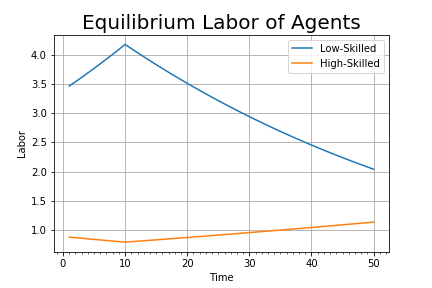
\includegraphics[width=\textwidth]{labor_agents}
        \label{fig:no_tax_labor}
      \end{subfigure}%
      ~
      \begin{subfigure}[b]{0.5\textwidth}
        \centering
        \caption{Equilibrium Consumption Allocation}
        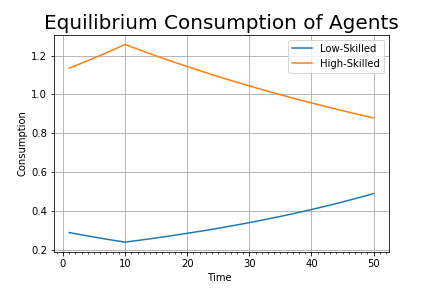
\includegraphics[width=\textwidth]{consumption_agents}
        \label{fig:no_tax_consump}
      \end{subfigure}%

      \begin{subfigure}[b]{0.5\textwidth}
        \centering
        \caption{Equilibrium Wages}
        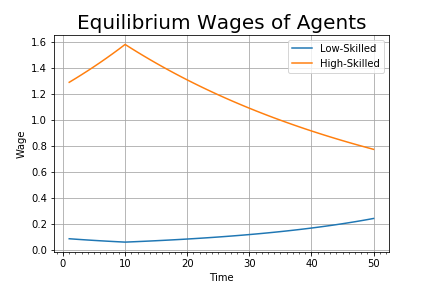
\includegraphics[width=\textwidth]{wage_agents}
        \label{fig:no_tax_wage}
      \end{subfigure}%
      ~
      \begin{subfigure}[b]{0.5\textwidth}
        \centering
        \caption{Aggregate Ouput Growth}
        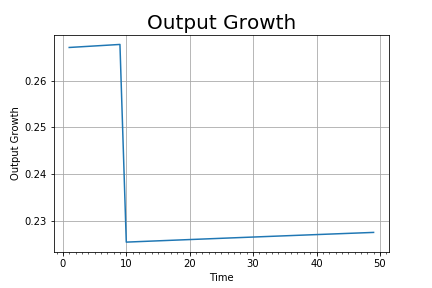
\includegraphics[width=\textwidth]{output_growth}
        \label{fig:no_tax_growth}
      \end{subfigure}
    \end{figure}

    \begin{figure}[H]
      \centering
      \caption{Equilibrium Labor, Consumption, Wages, and Aggregate Output Growth with Differently Skilled Agents, Anti-immigration Shock in Period 10 and Taxes}
      \label{fig:tax_same_r}
      \begin{subfigure}[b]{0.5\textwidth}
        \centering
        \caption{Equilibrium Labor Allocations}
        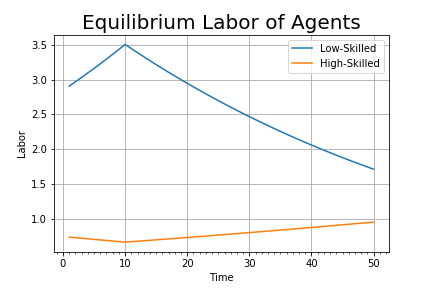
\includegraphics[width=\textwidth]{labor_agents_tax}
        \label{fig:tax_labor}
      \end{subfigure}%
      ~
      \begin{subfigure}[b]{0.5\textwidth}
        \centering
        \caption{Equilibrium Consumption Allocation}
        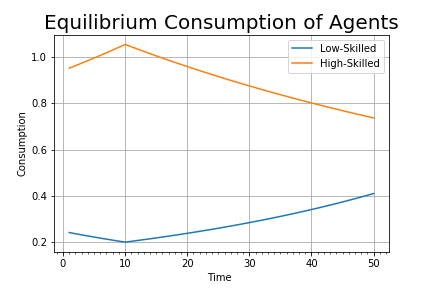
\includegraphics[width=\textwidth]{consumption_agents_tax}
        \label{fig:tax_consump}
      \end{subfigure}%

      \begin{subfigure}[b]{0.5\textwidth}
        \centering
        \caption{Equilibrium Wages}
        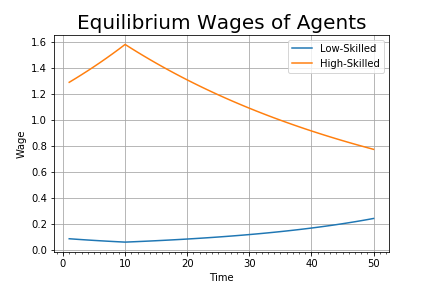
\includegraphics[width=\textwidth]{wage_agents_tax}
        \label{fig:tax_wage}
      \end{subfigure}%
      ~
      \begin{subfigure}[b]{0.5\textwidth}
        \centering
        \caption{Aggregate Ouput Growth}
        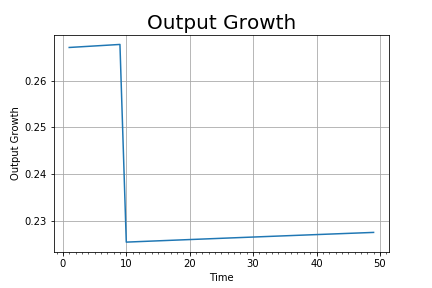
\includegraphics[width=\textwidth]{output_growth_tax}
        \label{fig:tax_growth}
      \end{subfigure}

      \begin{subfigure}[b]{0.5\textwidth}
        \centering
        \caption{Government Revenue Growth by Transfer Type}
        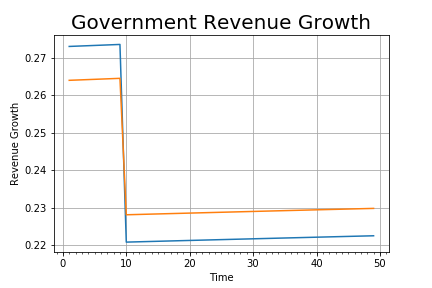
\includegraphics[width=\textwidth]{revenue_growth_tax}
        \label{fig:tax_transfer}
      \end{subfigure}%
      ~
      \begin{subfigure}[b]{0.5\textwidth}
        \centering
        \caption{Aggregate Government Revenue Growth}
        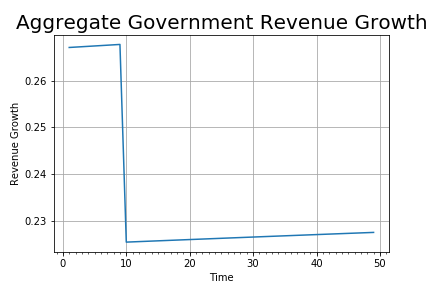
\includegraphics[width=\textwidth]{total_rev_growth_tax}
        \label{fig:tax_rev}
      \end{subfigure}
    \end{figure}

\begin{thebibliography}{1}
  \bibitem{nytimes} Peter Baker. {\em Trump Supports Plan to Cut Legal Immigration by Half}. 2017. Retrieved from https://www.nytimes.com/2017/08/02/us/politics/trump-immigration.html.
  \bibitem{timemag} Lisa Marie Segarra, David Johnson. {\em Find Out if President Trump Would Let You Immigrate to America}. 2017. Retrieved from http://time.com/4887574/trump-raise-act-immigration/.
  \bibitem{whitehouse} Office of the Press Secretary. {\em President Donald J. Trump Backs RAISE Act}. 2017. Retrieved from https://www.whitehouse.gov/the-press-office/2017/08/02/president-donald-j-trump-backs-raise-act.
  \bibitem{fortune} Benjamin Harris. {\em Why Your Economic Against Immigration is Probably Wrong}. 2017. Retrieved from http://fortune.com/2017/09/11/daca-immigration-economy-donald-trump/.
  \bibitem{politico} George J. Borjas. {\em Yes, Immigration Hurts American Workers}. 2016. Retrieved from https://www.politico.com/magazine/story/2016/09/trump-clinton-immigration-economy-unemployment-jobs-214216.
  \bibitem{havranek} Tomas Havranek. {\em Publication Bias in Measuring Intertemporal Substitution}. 2013.
  \bibitem{peterman} William B Peterman. {\em Reconciling Micro and Macro Estimates of the Frisch Labor Supply Elasticity: A Sensitivity Analysis}. 2014.
  \bibitem{BLS} Elka Torpey, Audrey Watson. {\em Education level and jobs: Opportunities by state}. 2014. Retrieved from https://www.bls.gov/careeroutlook/2014/article/education-level-and-jobs.htm.
  \bibitem{longhi} Simonetta Longhi, Peter Nijkamp, Jacques Poot. {\em A Meta-Analytic Assessment of the Effect of Immigration on Wages}. 2004.
  \bibitem{hercowitz} Zvi Hercowitz and Eran Yashiv. {\em A Macroeconomic Experiment in Mass Immigration}. 2002.
  \bibitem{ottaviano} Gianmarco I.P. Ottaviano, Giovanni Peri. {\em Rethinking the Effects of Immigration on Wages (working paper)}. 2006
  \bibitem{cortes} Patricia Cortes. {\em The Effect of Low-Skilled Immigration on U.S. Prices: Evidence from CPI Data}. 2008: Journal of Political Economy, Vol. 116, No. 3 pp 381-422.
  \bibitem{borjas03} George J. Borjas. {\em The Labor Demand Curve is Downward Sloping: Reexamining the Impact of Immigration on the Labor Market}. 2003.
  \bibitem{borjas14} George J. Borjas. {\em Immigration Economics}. 2014.
  \bibitem{clemens} Michael Clemens. {\em The Effect of Foreign Labor on Native Employment}. 2013.
  \bibitem{Friedberg} Rachel M. Friedberg. {\em The Impact of Mass Migration on the Israeli Labor Market}. 2001: The Quarterly Journal of Economics, Vol. 116, No. 4, pp. 1373-1408.
  \bibitem{Peri} Giovanni Peri. {\em The Effect of Immigration on Productivity: Evidence from US States}. 2009.
  \bibitem{kerr} William R. Kerr, William F. Lincoln. {\em The Supply Side of Innovation: H-1B Visa Reforms and US Ethnic Invention}. 2010.
  \bibitem{moser} Petra Moser, Alessandra Voena, Fabian Waldinger. {\em German Jewish Emigres and US Investion}. 2013.
  \bibitem{lisenkova} Katerina Lisenkova, Marcel Merette, Miguel Sanchez-Martinez. {\em Modelling Migration in an OLG Framework: the Case of UK Migration Policy}. 2013.
\end{thebibliography}

\end{document}
